% Sift whitepaper. Build: uv run python scripts/build_report.py  (XeLaTeX, run twice for references)
\documentclass[11pt,a4paper]{article}

% ---------------------------------------------------------------- fonts and layout
\usepackage{fontspec}
\setmainfont{Charter}
\setsansfont{Avenir Next}
\setmonofont{Menlo}[Scale=0.85]
\usepackage[a4paper,top=2.6cm,bottom=2.6cm,left=2.6cm,right=2.6cm,headheight=14pt]{geometry}
\usepackage{microtype}
\usepackage[table]{xcolor}
\usepackage{graphicx,calc,array,booktabs,etoolbox,float,needspace,enumitem,lastpage,tikz}
\usepackage[most]{tcolorbox}
\linespread{1.08}
\setlength{\parindent}{0pt}
\setlength{\parskip}{0.55em}
\setlength{\emergencystretch}{3em}
\providecommand{\tightlist}{\setlength{\itemsep}{0pt}\setlength{\parskip}{0pt}}
\setlist{leftmargin=1.4em,itemsep=2pt,topsep=4pt}

% ---------------------------------------------------------------- colours
\definecolor{accent}{HTML}{1F4E79}
\definecolor{accentdeep}{HTML}{13304F}
\definecolor{highlight}{HTML}{E07B24}
\definecolor{ink}{HTML}{1D2733}
\definecolor{muted}{HTML}{66717D}
\definecolor{rowshade}{HTML}{F1F4F8}
\definecolor{boxback}{HTML}{EEF3F9}

% ---------------------------------------------------------------- headings: numbered, sans, accent numbers
\usepackage{titlesec}
\titleformat{\section}{\sffamily\Large\bfseries\color{ink}}{\color{accent}\thesection}{0.7em}{}[\vspace{2pt}{\color{accent!25}\titlerule[0.8pt]}]
\titleformat{\subsection}{\sffamily\large\bfseries\color{ink}}{\color{accent}\thesubsection}{0.6em}{}
\titlespacing*{\section}{0pt}{3ex plus 1ex minus .2ex}{1.5ex}
\titlespacing*{\subsection}{0pt}{2.4ex plus .8ex minus .2ex}{0.8ex}
\pretocmd{\section}{\Needspace{10\baselineskip}}{}{}
\pretocmd{\subsection}{\Needspace{7\baselineskip}}{}{}

% ---------------------------------------------------------------- contents
\usepackage{tocloft}
\renewcommand{\cfttoctitlefont}{\sffamily\LARGE\bfseries\color{accent}}
\renewcommand{\cftsecfont}{\sffamily\bfseries}
\renewcommand{\cftsecpagefont}{\sffamily\bfseries}
\renewcommand{\cftsubsecfont}{\sffamily\small}
\renewcommand{\cftsubsecpagefont}{\sffamily\small}
\setlength{\cftbeforesecskip}{6pt}
\setcounter{tocdepth}{2}

% ---------------------------------------------------------------- header and footer
\usepackage{fancyhdr}
\pagestyle{fancy}
\fancyhf{}
\renewcommand{\sectionmark}[1]{\markboth{\thesection\quad #1}{}}
\fancyhead[L]{\sffamily\scriptsize\color{muted}\textbf{\color{accent}SIFT}\quad Whitepaper}
\fancyhead[R]{\sffamily\scriptsize\color{muted}\leftmark}
\fancyfoot[L]{\sffamily\scriptsize\color{muted}Twelve trading ideas, tested honestly on free data}
\fancyfoot[R]{\sffamily\scriptsize\color{muted}Page \textbf{\color{accent}\thepage} of \pageref{LastPage}}
\renewcommand{\headrulewidth}{0.4pt}
\renewcommand{\headrule}{\hbox to\headwidth{\color{accent!25}\leaders\hrule height \headrulewidth\hfill}}
\fancypagestyle{plain}{\fancyhf{}\fancyfoot[R]{\sffamily\scriptsize\color{muted}Page \textbf{\color{accent}\thepage} of \pageref{LastPage}}\renewcommand{\headrulewidth}{0pt}}

% ---------------------------------------------------------------- figures, tables, captions
\usepackage{caption}
\captionsetup{font={small,sf},labelfont={bf,color=accent},labelsep=colon,justification=raggedright,singlelinecheck=false,skip=6pt}
\captionsetup[table]{position=top,skip=4pt}
\renewcommand{\topfraction}{0.9}
\renewcommand{\bottomfraction}{0.7}
\renewcommand{\textfraction}{0.07}
\renewcommand{\floatpagefraction}{0.8}
\setcounter{topnumber}{2}
\setcounter{totalnumber}{3}
\AtBeginEnvironment{table}{\sffamily\footnotesize\setlength{\tabcolsep}{5pt}\renewcommand{\arraystretch}{1.25}\rowcolors{2}{rowshade}{white}}
\newcommand{\figterms}[1]{\par\vspace{3pt}{\raggedright\sffamily\scriptsize\color{muted}\textbf{Terms.} #1\par}}

% ---------------------------------------------------------------- boxes
\newtcolorbox{keybox}[1]{enhanced,breakable,colback=boxback,colframe=accent,boxrule=0pt,leftrule=3.5pt,arc=0pt,outer arc=0pt,
  left=12pt,right=12pt,top=8pt,bottom=8pt,before skip=10pt,after skip=12pt,fontupper=\sffamily\small\color{ink},
  title={#1},coltitle=accent,fonttitle=\sffamily\bfseries,colbacktitle=boxback,attach title to upper={\par\vspace{3pt}}}

% ---------------------------------------------------------------- links and metadata
\usepackage{hyperref}
\hypersetup{colorlinks=true,linkcolor=accent,urlcolor=accent,citecolor=accent,
  pdftitle={Sift: twelve trading ideas, tested honestly on free data},
  pdfsubject={A pre-registered negative-results whitepaper on short-term US stock strategies},
  pdfkeywords={backtesting, pre-registration, deflated Sharpe ratio, walk-forward, trading strategies}}
\urlstyle{same}

\begin{document}
\color{ink}

% ================================================================ title page
\begin{titlepage}
\thispagestyle{empty}
\begin{tikzpicture}[remember picture,overlay]
  \fill[accentdeep] (current page.north west) rectangle ([yshift=-3.6cm]current page.north east);
  \fill[highlight] ([yshift=-3.6cm]current page.north west) rectangle ([yshift=-3.75cm]current page.north east);
  \node[anchor=west,inner sep=0] (logo) at ([xshift=2.6cm,yshift=-1.8cm]current page.north west) {
\includegraphics[width=1.5cm]{figures/icon.pdf}};
  \node[anchor=west,text=white,font=\sffamily\bfseries\fontsize{24}{28}\selectfont] at ([xshift=0.4cm]logo.east) {Sift};
  \node[anchor=east,text=white!80!accent,font=\sffamily\small\bfseries] at ([xshift=-2.6cm,yshift=-1.8cm]current page.north east) {WHITEPAPER \quad\textbar\quad VERSION 1.0};
\end{tikzpicture}

\vspace*{3.6cm}
{\sffamily\small\bfseries\color{highlight} RESEARCH WHITEPAPER\par}
\vspace{0.35cm}
{\sffamily\bfseries\fontsize{32}{38}\selectfont\color{ink} Twelve trading ideas,\\ tested honestly on free data\par}
\vspace{0.45cm}
{\sffamily\Large\color{muted} A pre-registered negative-results study of short-term US stock strategies\par}
\vspace{0.9cm}
{\sffamily\small\color{ink}\textbf{Malek Khalifa}\quad\textcolor{muted}{\textbar}\quad 6 November 2026\quad\textcolor{muted}{\textbar}\quad \href{https://github.com/Malekhalifa/sift}{github.com/Malekhalifa/sift}\par}
\vspace{0.8cm}
{\color{accent!25}\rule{\linewidth}{0.8pt}}\par
\vspace{0.3cm}
{\sffamily\bfseries\color{accent} Abstract\par}
\vspace{0.1cm}
{\small
Trading strategies spread online because they are easy to describe and easy to believe. This paper asks whether any of
them survive a fair test, starting from \$0 and using only free data. It describes \textbf{Sift}, a research pipeline that
downloads market data, turns each trading idea into exact rules, simulates the trades with realistic costs, and judges the
results with checks designed to catch luck: pre-registration of every protocol before it runs, walk-forward testing,
an untouched holdout, a count of every configuration tried with a Deflated Sharpe Ratio, a comparison against simply
holding the market, and replication on unseen stocks. Twelve ideas were tested on up to 410 US stocks from 2016 to 2024:
opening-range breakouts and fades, RSI reversion, trend pullbacks, earnings drift, insider buying, two indicator bots
popular in online videos, volume-conditioned rules, presidential social-media posts and Pentagon contract awards.
\textbf{None met all of its pre-registered criteria.} The ideas that looked strongest were either the market's own rise
or luck that did not repeat on new stocks. The contribution is a method and a set of lessons about how backtests flatter
themselves, not a strategy.\par}
\vfill
{\sffamily\scriptsize\color{muted}
\textbf{Disclaimer.} A personal research project. It is not investment advice and recommends no security or strategy;
no real money was traded. The code, analysis and drafting were done with an AI coding assistant; every number comes from
results recorded in the project repository, whose commit history records when each protocol was written.\par}
\end{titlepage}

% ================================================================ contents
\tableofcontents
\clearpage

% ================================================================ executive summary
\section*{Executive summary}
\addcontentsline{toc}{section}{Executive summary}
\markboth{Executive summary}{}

Sift was built to answer a practical question: can a retail trader with no capital and only free data find a
short-term edge in US stocks, and prove it before risking money? Twelve ideas were each turned into exact rules, written
down before testing, and judged out of sample by seven fixed criteria. The 2025 to 2026 data was locked away for a final
check that no idea earned.

\begin{center}

\begin{tikzpicture}
  \foreach \x/\num/\lab in {0/12/ideas tested, 3.15/0/passed every check, 6.3/298/configurations counted, 9.45/410/US stocks at most, 12.6/9/years of data}
  {
    \node[anchor=north west,inner sep=0,text=accent,font=\sffamily\bfseries\fontsize{24}{28}\selectfont] at (\x,0) {\num};
    \node[anchor=north west,inner sep=0,text width=2.7cm,text=muted,font=\sffamily\scriptsize] at (\x,-0.95) {\lab};
  }
\end{tikzpicture}
\end{center}

\begin{keybox}{Key findings}
\begin{itemize}[leftmargin=1.2em]
\item \textbf{No idea passed.} The two closest, earnings drift and a high-volume rule, each passed five checks and then
      failed the decisive ones.
\item \textbf{Apparent edges were usually the market.} Long-only rules looked positive because stocks rose from 2019 to 2024;
      after subtracting the market, insider buying fell from +0.028R to −0.079R per trade.
\item \textbf{Luck did not replicate.} Earnings drift (+0.156R on 149 stocks) fell to +0.025R on 250 stocks it had never
      seen.
\item \textbf{Costs were not the reason.} Several ideas showed no edge even with trading costs set to zero, and the largest
      tests had about 100,000 trades, so the negatives are precise.
\end{itemize}
\end{keybox}

\textbf{What this means.} For traders, a strategy shown online is one run, chosen after the fact; it should be held to the
same tests before any money follows it. For anyone building backtests, the four safeguards that mattered most here are
cheap to adopt: write the rules down first, count every try, subtract the market, and repeat the test on data that played
no part in choosing the rule. For this project, the free-data, short-term route is closed; the method remains in place for
the next question.

\textbf{How to read this paper.} Section~\ref{sec:intro} explains why Sift was built and how it works,
Section~\ref{sec:ideas} describes the twelve ideas in plain words, Section~\ref{sec:method} sets out the method,
Sections~\ref{sec:results} and~\ref{sec:discussion} report and interpret the results, and Section~\ref{sec:limits} states
what the study cannot show. A glossary of every abbreviation is in Appendix~\ref{app:glossary}.

\clearpage
\section{Introduction}\label{sec:intro}

\subsection{Motivation}\label{sec:motivation}

Strategies spread online because they are easy to describe and easy to believe: a bot that doubled a small account
overnight, a pair of indicators with a high win rate, a screenshot of a good week. What is missing is a fair test. Two
traps make almost any idea look good:

\begin{itemize}
\tightlist
\item
  \textbf{Selection luck.} Try enough rules on one stretch of history and some will fit it by chance. This is called
  overfitting, or data-snooping, and the best-looking result of many tries is the one most likely to be luck.
\item
  \textbf{The market's own rise.} In a period when stocks go up, almost any rule that buys will make money. That is not skill.
\end{itemize}

The goal was therefore twofold: build a pipeline that could find a short-term edge in US stocks, and make it hard for the
pipeline to fool its builder. The rule was: \textbf{no real money until an idea has proved itself on data it was not tuned on.}
Starting capital is \$0, so everything uses free data and paper trading. The name, Sift, is the method: put each idea on a
sieve and see what stays behind. So far, mostly chaff.

\subsection{How Sift works}\label{sec:how}

Sift has five parts, in the order data moves through them:

\begin{enumerate}
\def\labelenumi{\arabic{enumi}.}
\tightlist
\item
  \textbf{Data.} A recorder downloads free market data (Alpaca's free tier gives consolidated-tape bars back to 2016), SEC
  filings, government contract records and public archives of posts, and stores them locally. Stock splits are applied
  when data is read, so a new split never corrupts history.
\item
  \textbf{Strategies.} Each idea is turned into exact rules that output trade signals: a direction, an entry, a stop-loss and a
  profit target, with the target fixed at 1.5 times the risk.
\item
  \textbf{Backtest engine.} It replays history trade by trade with realistic conventions: orders fill at the next bar's open plus
  slippage, a stop wins when a bar touches both stop and target, and gaps fill at the open. Results are measured in R, the
  profit as a multiple of the amount risked.
\item
  \textbf{Statistics.} Parameters are chosen on earlier years only and judged on later ones (walk-forward). Every configuration
  tried is logged, and a Deflated Sharpe check asks whether a result survives that many attempts. The market is subtracted,
  and promising results must repeat on stocks the rule never saw.
\item
  \textbf{Paper trading.} A loop that places orders on a broker's paper account was built and tested for plumbing, ready for the day an
  idea passes. None did, so nothing was ever run for evidence.
\end{enumerate}

\begin{figure}[tbp]
\centering
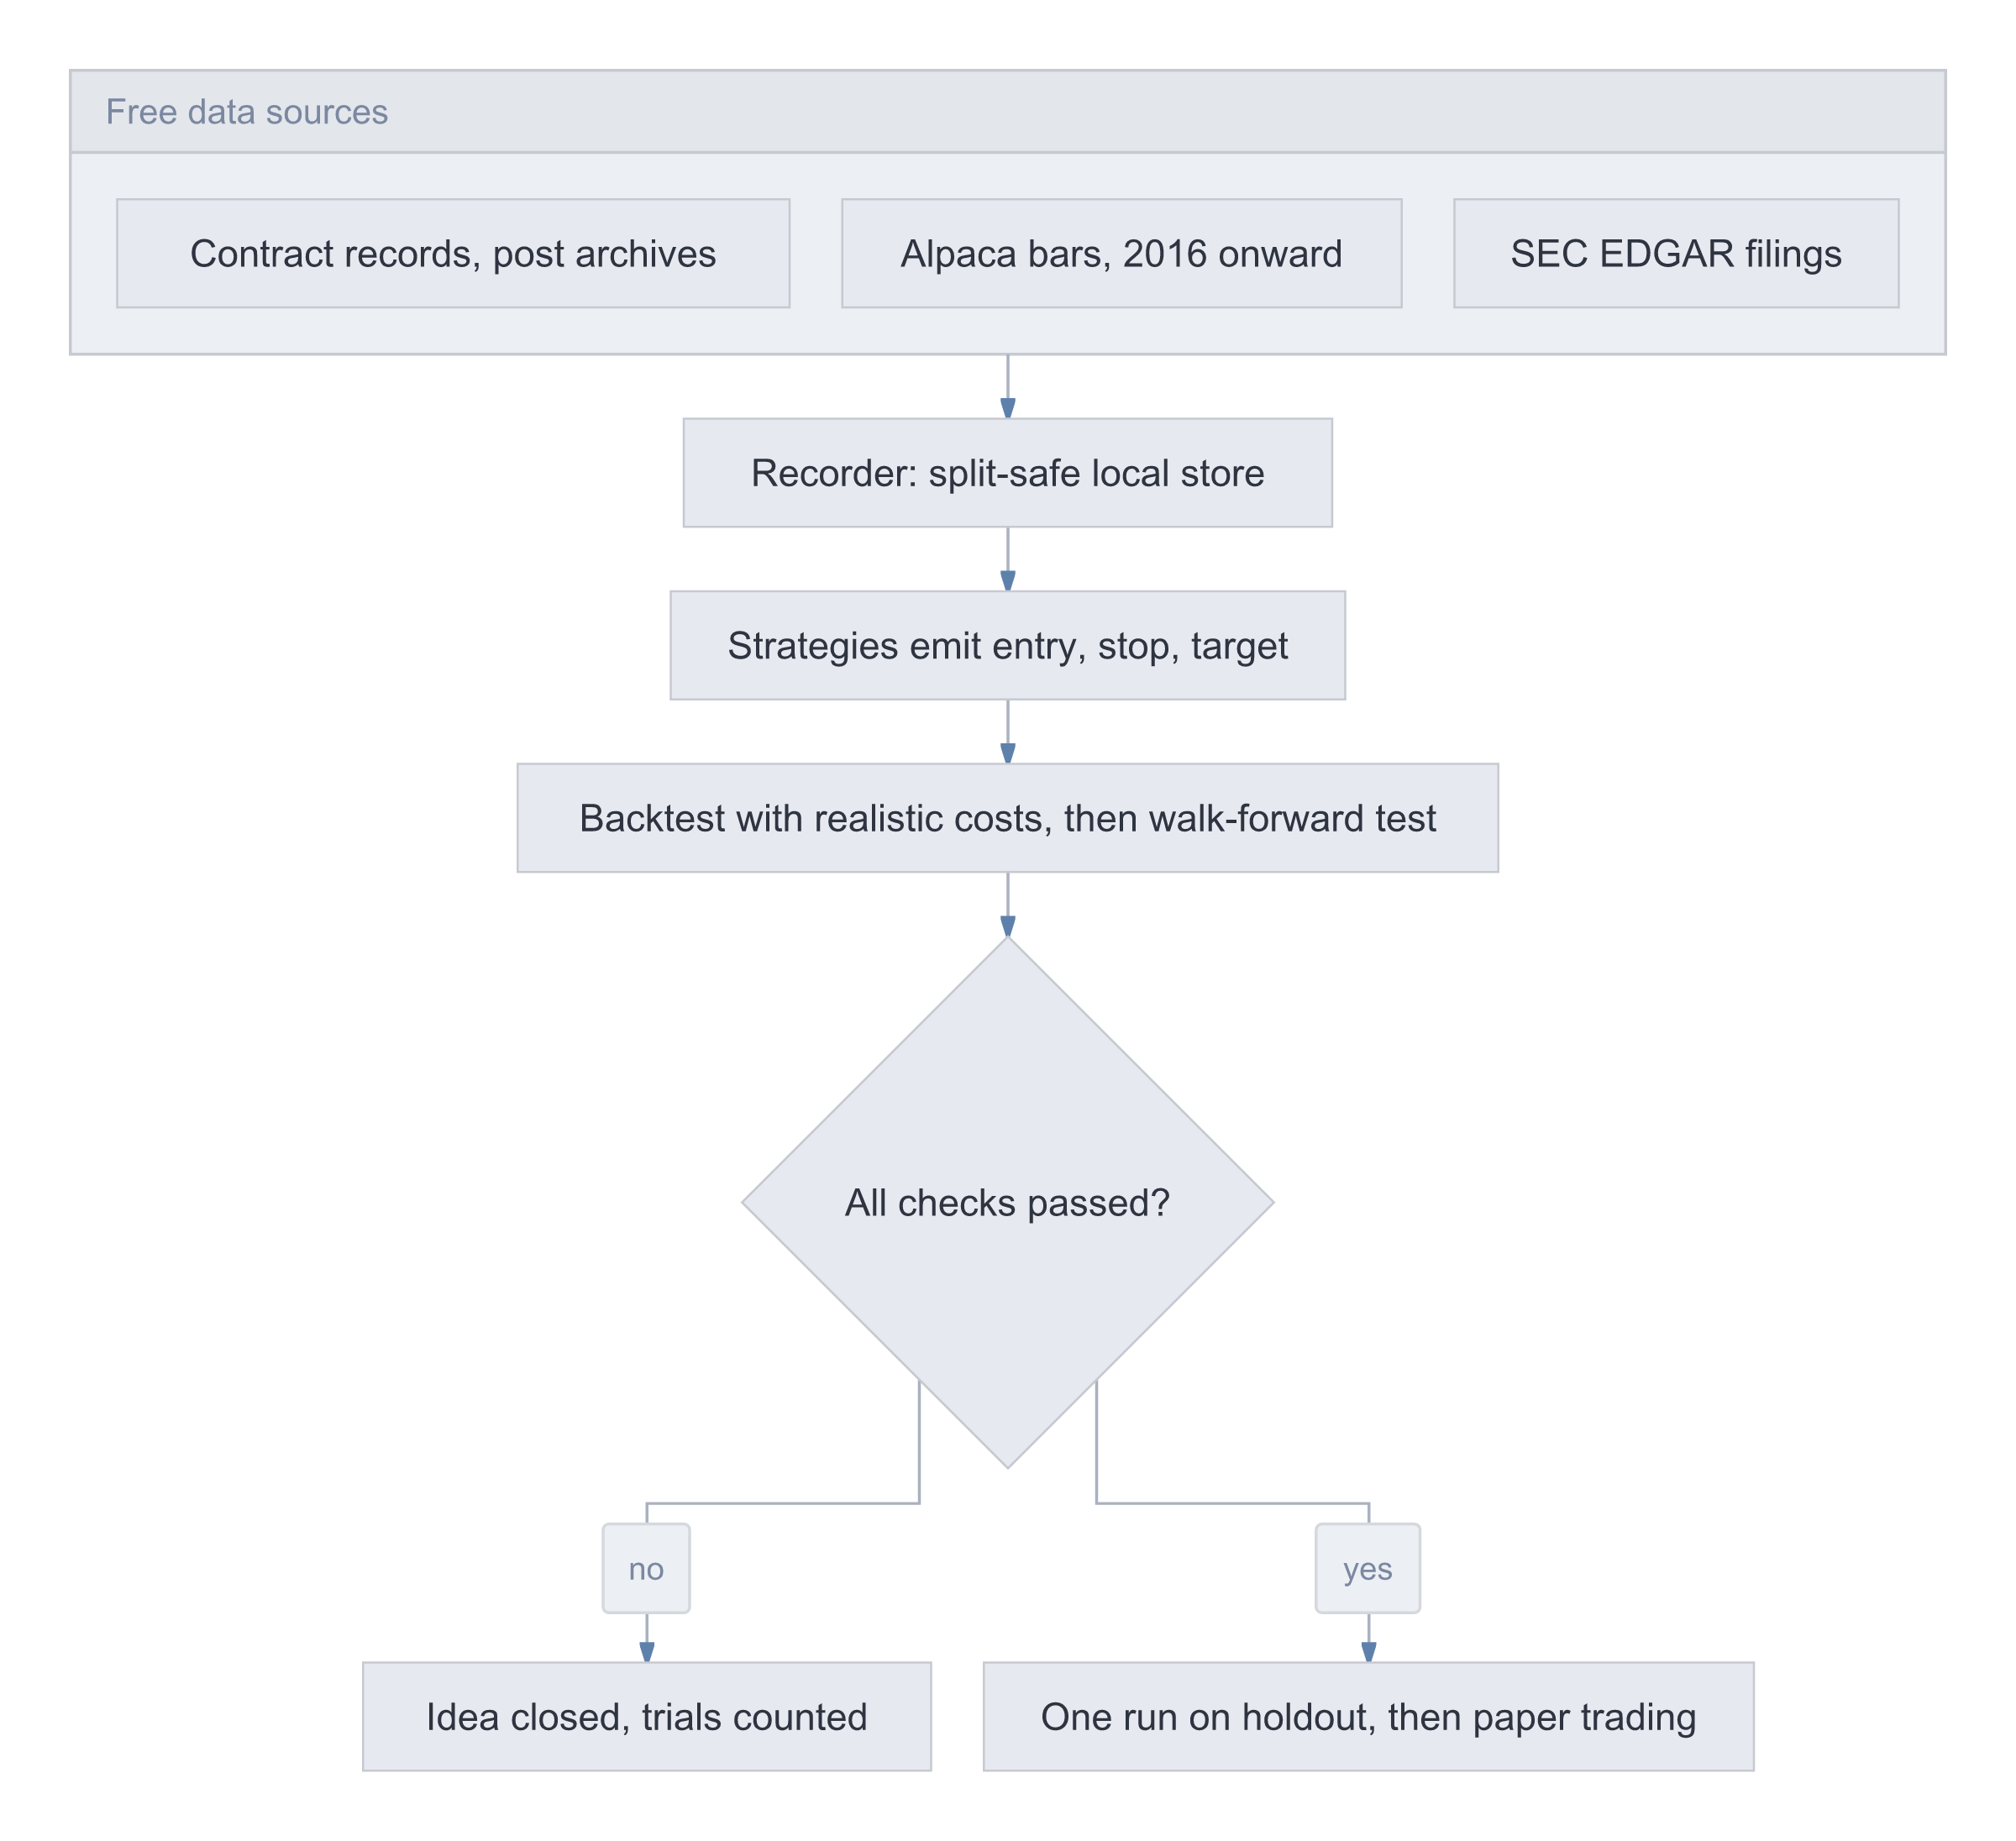
\includegraphics[width=0.80\linewidth]{figures/pipeline.png}
\caption[The pipeline]{The pipeline. Data flows from free sources through a split-safe store into strategies and a cost-aware backtest; only an idea that passes every check reaches the holdout, and only after that paper trading.}
\label{fig:pipeline}
\figterms{Alpaca = a US broker whose free tier supplies the price data. Bars = price candles (open, high, low, close, volume) for one time period. SEC = the US Securities and Exchange Commission; EDGAR = its public database of company filings. Split-safe = stock splits are adjusted when data is read. Stop = an order that exits a losing trade; target = an order that exits a winning trade. Backtest = replaying history to see what a rule would have done. Walk-forward = choosing settings on earlier years and testing them on later ones. Holdout = recent data kept unseen until the end. Paper trading = simulated trading on a broker's practice account. Trials counted = every configuration tried is logged.}
\end{figure}

The work was organised as one \textbf{milestone per idea}. For each, a protocol (the exact rules, the parameter grid and the pass
criteria) was written and committed to version control first; the test was then run once, and the result was recorded
whatever it showed. The commit history therefore proves the order. The code, the analysis and the drafting were done with an
AI coding assistant; the decisions, and every number in this report, trace back to results recorded in the repository.

\subsection{Constraints fixed at the start}\label{sec:constraints}

\begin{itemize}
\tightlist
\item
  US stocks, short-term horizons (minutes to a few weeks), a fixed 1:1.5 risk-to-reward bracket on trades.
\item
  Start with \$0 of capital. Free data only: Alpaca's free tier (consolidated-tape bars from 2016, 15 minutes delayed),
  SEC EDGAR filings, USAspending.gov, public archives of presidential posts.
\item
  Universe chosen by a fixed rule (median dollar volume in Q1 2016), never by hand: 10 large caps, then 50, 150 and 250
  further stocks (about 410 in total).
\end{itemize}

\section{The twelve ideas}\label{sec:ideas}

Each idea is a belief about how prices behave. A test asks one question: if I had acted on that belief with fixed rules, would
I have made money after costs, and was that more than just holding the market? The ideas came from four places: classic
day-trading lore (ideas 1 to 4), academic research (5, 6, 11 and 12), indicator ``bots'' shown in online videos (9 and 10), and
the intuition that politics moves stocks (7 and 8).

\subsection{Short-term price patterns (minutes to hours, 5-minute bars)}\label{short-term-price-patterns-minutes-to-hours-5-minute-bars}

\begin{enumerate}
\def\labelenumi{\arabic{enumi}.}
\tightlist
\item
  \textbf{Opening-range breakout.} \emph{The belief:} the first minutes of the trading day set a range, and when price closes beyond it,
  the move tends to continue. \emph{The test:} trade in the direction of the break with a stop and a target at 1.5 times the
  risk, and close the trade by the end of the day. Optional filters were unusual volume, an overnight gap and the market's
  trend. Tried on 10 large stocks, then on 50 fresh ones.
\item
  \textbf{Failed-breakout fade.} \emph{The belief:} a breakout that fails, with price closing back inside the range, traps the traders
  who bought it and reverses. \emph{The test:} bet against the failed move, with the stop just beyond its extreme.
\end{enumerate}

\subsection{Daily swing trades (days to weeks, daily bars)}\label{daily-swing-trades-days-to-weeks-daily-bars}

\begin{enumerate}
\def\labelenumi{\arabic{enumi}.}
\setcounter{enumi}{2}
\tightlist
\item
  \textbf{RSI(2) mean reversion.} \emph{The belief:} after a sharp two-day fall a stock tends to bounce within days, and to fall back
  after a sharp rise. \emph{The test:} buy when the 2-day RSI, a gauge of very short-term momentum, is extremely low and sell
  short when it is extremely high, optionally only in the direction of the 200-day trend.
\item
  \textbf{20/200-day pullback.} \emph{The belief:} in an established uptrend, a dip back to the 20-day average is a chance to buy
  cheaply, and the reverse in a downtrend. \emph{The test:} trade the first close back to the 20-day average while the
  20-day and 200-day averages agree on the trend.
\end{enumerate}

\subsection{Events and news (daily bars)}\label{events-and-news-daily-bars}

\begin{enumerate}
\def\labelenumi{\arabic{enumi}.}
\setcounter{enumi}{4}
\tightlist
\item
  \textbf{Earnings drift.} \emph{The belief:} when a company reports results and its stock jumps or falls by an unusual amount, it keeps
  moving the same way for days or weeks. \emph{The test:} take the timing from the exact moment of the SEC filing of each
  earnings release, measure the market-adjusted reaction in multiples of the stock's normal daily range, and follow (or
  fade) reactions of one to three ranges. The drift is reported to have faded outside the smallest stocks \cite{martineau2022}.
\item
  \textbf{Insider buying.} \emph{The belief:} when company officers and directors buy shares with their own money they may know something
  the market does not, especially if the purchase is out of character (``opportunistic'') rather than a habit (``routine'').
  \emph{The test:} trade clusters of purchases at the open after the public SEC filing, with the routine and opportunistic split
  from an academic paper by Cohen, Malloy and Pomorski \cite{cohen2012}.
\item
  \textbf{Presidential posts.} \emph{The belief:} when the US president praises or attacks a listed company on social media, its stock
  moves, and a slower trader can still profit. \emph{The test:} find posts that name a company (tweets 2016 to 2018, Truth Social
  2022 to 2024), take their tone from fixed word lists, enter at the first open after the post, hold five sessions.
\item
  \textbf{Pentagon contract awards.} \emph{The belief:} a large defence contract lifts the stock of the winner. \emph{The test:} use awards of
  \$100 million or more to seven listed contractors from USAspending.gov, buy at the open two sessions after the award
  date and hold five sessions.
\end{enumerate}

\subsection{Indicator bots popular in online videos (5-minute bars)}\label{indicator-bots-popular-in-online-videos-5-minute-bars}

\begin{enumerate}
\def\labelenumi{\arabic{enumi}.}
\setcounter{enumi}{8}
\tightlist
\item
  \textbf{UT Bot + Schaff Trend Cycle.} \emph{The belief:} a trailing-stop indicator (UT Bot) flipping direction marks the start of a
  trend, and a second indicator (Schaff Trend Cycle) confirms it. \emph{The test:} the common open-source definitions, 18 settings,
  including the video's asymmetric setup with different long and short parameters.
\item
  \textbf{Supertrend + Waddah Attar Explosion.} \emph{The belief:} a trend line (Supertrend) agreeing with a momentum-surge indicator
  (Waddah Attar) marks high-quality entries, optionally only when the market is trending (ADX or Choppiness filter).
  \emph{The test:} 12 settings, with the stop distance used in the video.
\end{enumerate}

\subsection{Volume (daily bars)}\label{volume-daily-bars}

\begin{enumerate}
\def\labelenumi{\arabic{enumi}.}
\setcounter{enumi}{10}
\tightlist
\item
  \textbf{Volume-dry-up reversal.} \emph{The belief:} a stock that fell (or rose) against the market over a week on shrinking volume was
  pushed by impatient traders rather than news, and tends to snap back. \emph{The test:} trade against such moves of two to
  three daily ranges, with and without the volume condition.
\item
  \textbf{High-volume continuation.} \emph{The belief:} a stock whose volume is the highest in weeks is receiving new attention and tends
  to drift upward over the following weeks. \emph{The test:} buy on the highest-volume day of the last 20 or 50 sessions, long only.
\end{enumerate}

One more test is a side question, not an idea (Section \ref{sec:trend}): whether a 200-day trend filter makes simply holding the market
safer.

\textbf{What was expected.} Where a protocol stated a chance of passing in advance, it was low: about 3 to 5\% for each indicator
bot, about 10\% for insider buying, 12\% and 8\% for the two volume ideas, and 3\% and 2\% for the two political ones. The
outcomes were consistent with those priors, and none of the tests was chosen because it was expected to win.

\section{Methodology}\label{sec:method}

Most backtests that look good are noise that was selected. The framework was built to make that hard: Figure \ref{fig:method} shows the
method applied to every idea, and Table \ref{tbl:safeguards} lists its safeguards.

\begin{table}[tbp]
\centering
\caption{Safeguards built into every test.}\label{tbl:safeguards}
\begin{tabular}{@{}
  >{\raggedright\arraybackslash}p{(\linewidth - 2\tabcolsep) * \real{0.2273}}
  >{\raggedright\arraybackslash}p{(\linewidth - 2\tabcolsep) * \real{0.7727}}@{}}
\toprule
\begin{minipage}[b]{\linewidth}\raggedright
Safeguard
\end{minipage} & \begin{minipage}[b]{\linewidth}\raggedright
What it does
\end{minipage} \\
\midrule
\textbf{Pre-registration} & For each test the protocol, parameter grid and pass criteria were committed to version control before the run. The commit history shows the order, so it cannot be quietly changed afterwards. \\
\textbf{Walk-forward, out of sample} & Parameters are chosen on earlier years only and judged on the next. Test years were 2019 to 2024. \\
\textbf{Untouched holdout} & Data from 2025 onward is kept for a single final run, and only for an idea that has already passed everything. The code refuses to read it without an explicit flag. No analysis has read it. \\
\textbf{Trial counting and Deflated Sharpe} & Every configuration tried is logged (298 in total). The Deflated Sharpe Ratio (Bailey and L\textquotesingle opez de Prado \cite{bailey2014}) asks whether a result still stands after paying for the number of attempts. \\
\textbf{Realistic fills and costs} & Next-bar fills, stops assumed hit first when a bar is ambiguous, gaps filled at the open, per-share slippage on market fills, limit targets that must trade through to fill, stock splits handled at read time, one open trade per symbol. A stress test doubles costs. \\
\textbf{Market-adjusted check} & Added after earnings drift: each trade's result minus what holding SPY (the exchange-traded fund that tracks the S\&P 500 index) the same way over the same dates would have earned. \\
\textbf{Replication on unseen stocks} & A single frozen setting is run once on stocks that took no part in choosing it. \\
\bottomrule
\end{tabular}
\end{table}

\textbf{Pass criteria (all must hold):} at least 300 out-of-sample trades; the 95\% interval of expectancy above zero; Deflated
Sharpe at least 0.95; positive in at least 4 of 6 test years; still positive at double costs; at least 70\% of
neighbouring parameter settings positive; and, from M8 on, a market-adjusted interval above zero. A test with too few
trades is ``inconclusive'', not a pass.

A note on units: \textbf{R} is profit measured in the amount risked on the trade. +0.1R means the average trade made 10\% of
what it risked, after costs.

\subsection{Reading a result}\label{reading-a-result}

A worked example shows why the 1.5 times target matters. Suppose each trade risks \$100, the distance from the entry to the
stop. A winner that reaches the target earns \$150, which is +1.5R; a loser costs \$100, which is −1R. The break-even win rate
is therefore 40\% (0.4 x 1.5 - 0.6 x 1 = 0). A rule can win 46\% of its trades and still earn almost nothing: the insider-buying
test won 45.9\%, but its wins averaged +1.26R and its losses −1.02R, which nets to +0.03R before looking at the market.

A test's result is its average R per trade, the expectancy, with a 95\% confidence interval: the range in which the true
average very probably lies. ``+0.028R ±0.078'' means the true value could be anywhere from −0.050R to +0.106R, so it cannot
be told apart from zero. A result counts as an edge only when the whole interval sits above zero.

\subsection{How a trade is simulated}\label{how-a-trade-is-simulated}

Each strategy emits a signal when a bar closes. The simulator then follows a fixed script, so that a rule cannot flatter itself:

\begin{enumerate}
\def\labelenumi{\arabic{enumi}.}
\tightlist
\item
  \textbf{Entry.} A market order is filled at the next bar's open plus slippage, an assumed cost per share: one cent on liquid
  stocks, two cents on mid-sized ones, doubled in the stress test.
\item
  \textbf{Exit.} The stop and the target are set when the signal fires. If one bar touches both, the loss is counted, the cautious
  assumption. If price gaps past the stop, the exit is at the gap price, not at the stop. A profit target fills only when
  price trades through it, not when it merely touches it. Intraday trades are closed by 15:55 New York time; daily trades
  are closed at the close after a maximum holding period.
\item
  \textbf{Measurement.} Every simulated trade is scored in R, before any position sizing, so the statistics do not depend on how
  much money is assumed to be in the account. A separate portfolio view sizes each trade to risk 1\% of the account under
  leverage and position caps.
\end{enumerate}

\subsection{How walk-forward works}\label{how-walk-forward-works}

Settings are never judged on the data that chose them. For each test year, the best-looking setting is picked using only
earlier years and then run on the year it has not seen (Table \ref{tbl:walkforward}):

\begin{table}[tbp]
\centering
\caption{Walk-forward schedule: each test year is judged with a setting chosen on earlier years only.}\label{tbl:walkforward}
\begin{tabular}{@{}ll@{}}
\toprule
Test year & Setting chosen using data from \\
\midrule
2019 & 2016 to 2018 \\
2020 & 2016 to 2019 \\
2021 & 2016 to 2020 \\
2022 & 2016 to 2021 \\
2023 & 2016 to 2022 \\
2024 & 2016 to 2023 \\
\bottomrule
\end{tabular}
\end{table}

The six test years are joined into one out-of-sample record, and that record is what the results below report. ``Best-looking''
means the highest average R minus one standard error, so a setting that did well on very few trades is penalised.

\subsection{What the Deflated Sharpe check asks}\label{what-the-deflated-sharpe-check-asks}

The Sharpe ratio measures return per unit of risk. If hundreds of settings are tried, the best of them will have an
impressive Sharpe ratio by luck alone, even if every one is worthless. The Deflated Sharpe Ratio estimates the probability
that the best result is genuine after discounting for the number of attempts (298 in total here); the criterion is at least
0.95. For a single frozen setting tested once on new stocks (M8) there is nothing to deflate for, so the check reduces to the
probability that the true Sharpe ratio is above zero.

\begin{figure}[tbp]
\centering
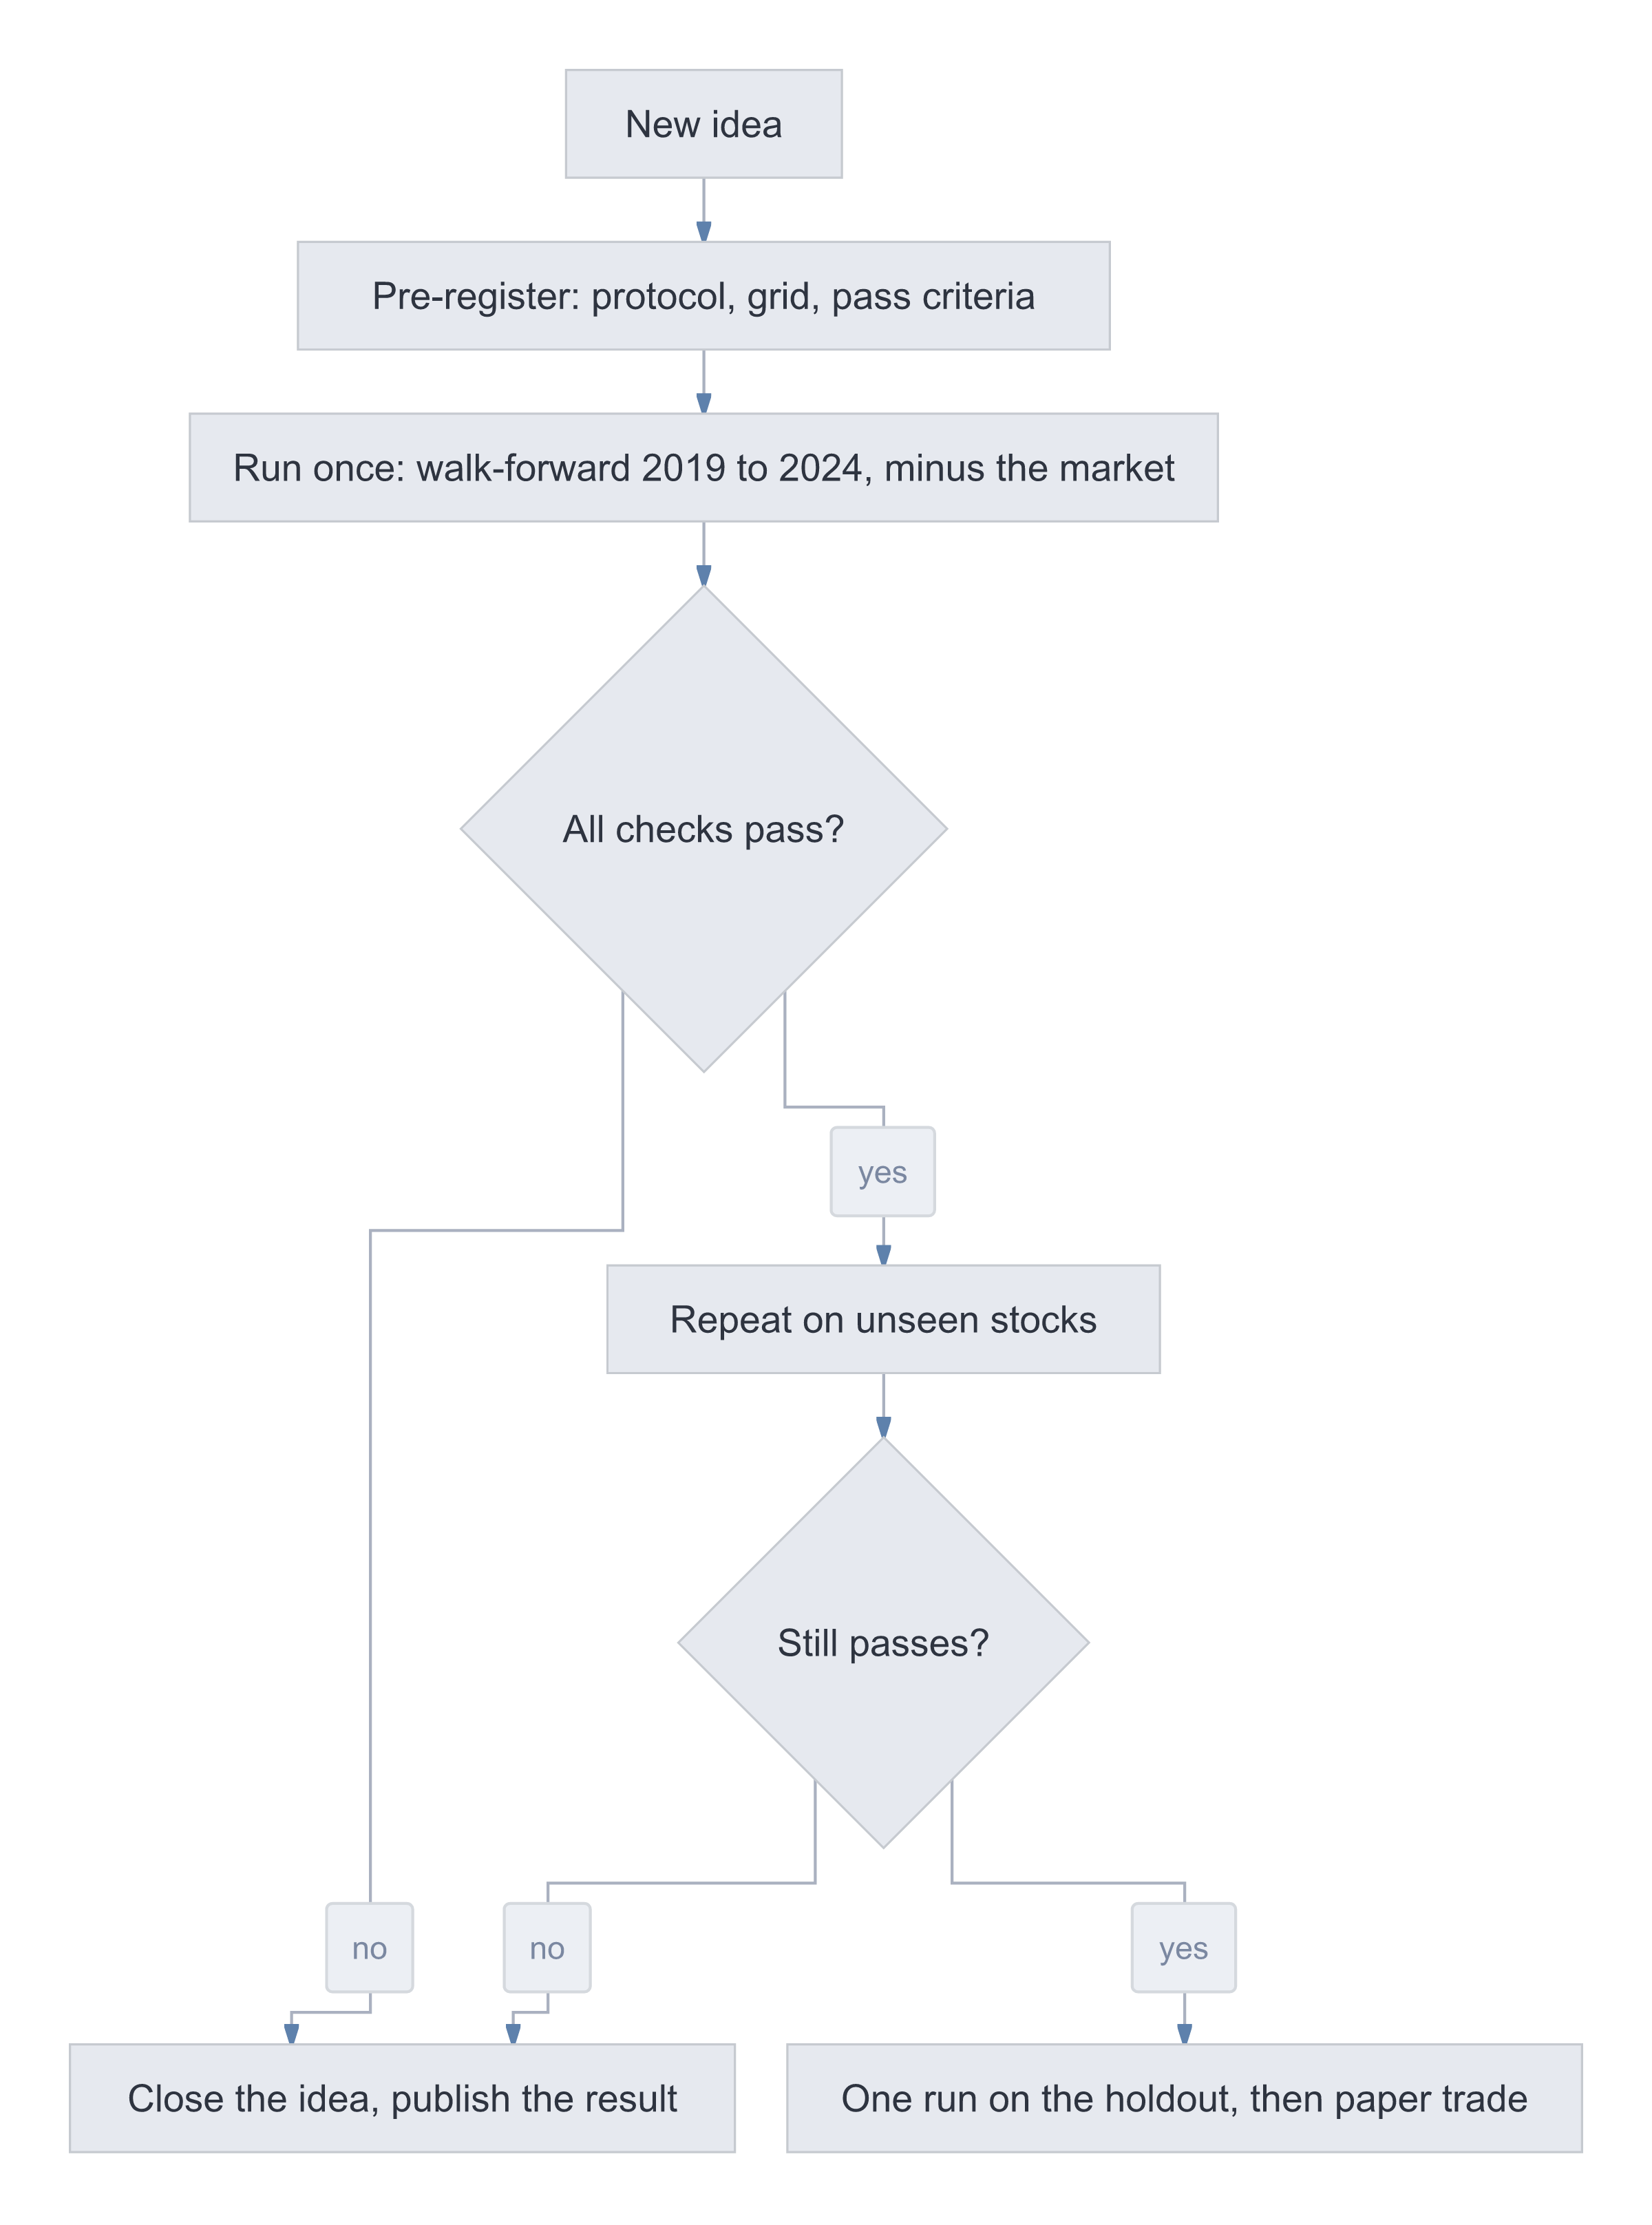
\includegraphics[width=0.66\linewidth]{figures/method.png}
\caption[The method applied to every idea]{The method applied to every idea. Failing at any gate closes the idea and the result is published either way.}
\label{fig:method}
\figterms{Pre-register = write down and commit the rules before running anything. Protocol = the exact rules and pass criteria; grid = the list of parameter settings to try. Walk-forward = settings chosen on earlier years, tested on later ones (Section \ref{sec:method}). Minus the market = subtract what simply holding the market earned over the same dates. Every trial counted = each setting tried is logged and the final statistics account for the number of tries. Checks = the seven pass criteria listed in Section \ref{sec:method}. Unseen stocks = stocks that took no part in choosing the setting. Holdout = data from 2025 onward, kept unread.}
\end{figure}

\section{Results}\label{sec:results}

Table \ref{tbl:results} gives each idea's out-of-sample result and how many of its pre-registered checks it passed; Figure \ref{fig:forest} shows the
same results as a picture, with their 95\% intervals.

\begin{table}[tbp]
\centering
\caption{Out-of-sample results of every test, with the number of pre-registered checks passed.}\label{tbl:results}
\begin{tabular}{@{}
  >{\raggedright\arraybackslash}p{(\linewidth - 8\tabcolsep) * \real{0.0988}}
  >{\raggedright\arraybackslash}p{(\linewidth - 8\tabcolsep) * \real{0.3086}}
  >{\raggedright\arraybackslash}p{(\linewidth - 8\tabcolsep) * \real{0.2469}}
  >{\raggedright\arraybackslash}p{(\linewidth - 8\tabcolsep) * \real{0.2469}}
  >{\raggedright\arraybackslash}p{(\linewidth - 8\tabcolsep) * \real{0.0988}}@{}}
\toprule
\begin{minipage}[b]{\linewidth}\raggedright
Milestone
\end{minipage} & \begin{minipage}[b]{\linewidth}\raggedright
Idea
\end{minipage} & \begin{minipage}[b]{\linewidth}\raggedright
Data
\end{minipage} & \begin{minipage}[b]{\linewidth}\raggedright
Out-of-sample result (95\% interval)
\end{minipage} & \begin{minipage}[b]{\linewidth}\raggedright
Checks passed
\end{minipage} \\
\midrule
M4 & Opening-range breakout & 10 large caps, 5-min bars & +0.065R ±0.114 & 3 of 6 \\
M4 & Failed-breakout fade & same & −0.000R ±0.042 & 1 of 6 \\
M4b & Opening-range breakout & 50 fresh stocks & −0.046R ±0.028 & 1 of 6 \\
M6 & RSI(2) mean reversion & 50 stocks, daily & −0.026R ±0.021 & 1 of 6 \\
M6 & 20/200-day pullback & 50 stocks, daily & −0.032R ±0.028 & 1 of 6 \\
M7 & Earnings drift (SEC filing times) & 149 stocks, daily & +0.156R ±0.099 & 5 of 6 \\
M8 & M7's frozen setting, replicated & 250 unseen stocks & +0.025R ±0.077 & 2 of 7 \\
M9 & UT Bot + Schaff Trend Cycle & 50 stocks, 5-min & −0.038R ±0.006 & 1 of 6 \\
M9 & Supertrend + Waddah Attar & 50 stocks, 5-min & −0.042R ±0.005 & 1 of 6 \\
M10 & Insider buying (SEC Form 4) & 407 stocks, daily & +0.028R ±0.078 & 3 of 7 \\
M11 & Volume-dry-up reversal & 409 stocks, daily & −0.008R ±0.010 & 1 of 7 \\
M11 & High-volume continuation & 409 stocks, daily & +0.100R ±0.019 & 5 of 7 \\
M12 & Presidential posts naming a listed company & 133 events & −0.05\% ±0.60 per event & 1 of 4 \\
M12 & Large Pentagon awards to listed primes & 933 events & −0.10\% ±0.27 per event & 1 of 4 \\
\bottomrule
\end{tabular}
\end{table}

\begin{figure}[tbp]
\centering
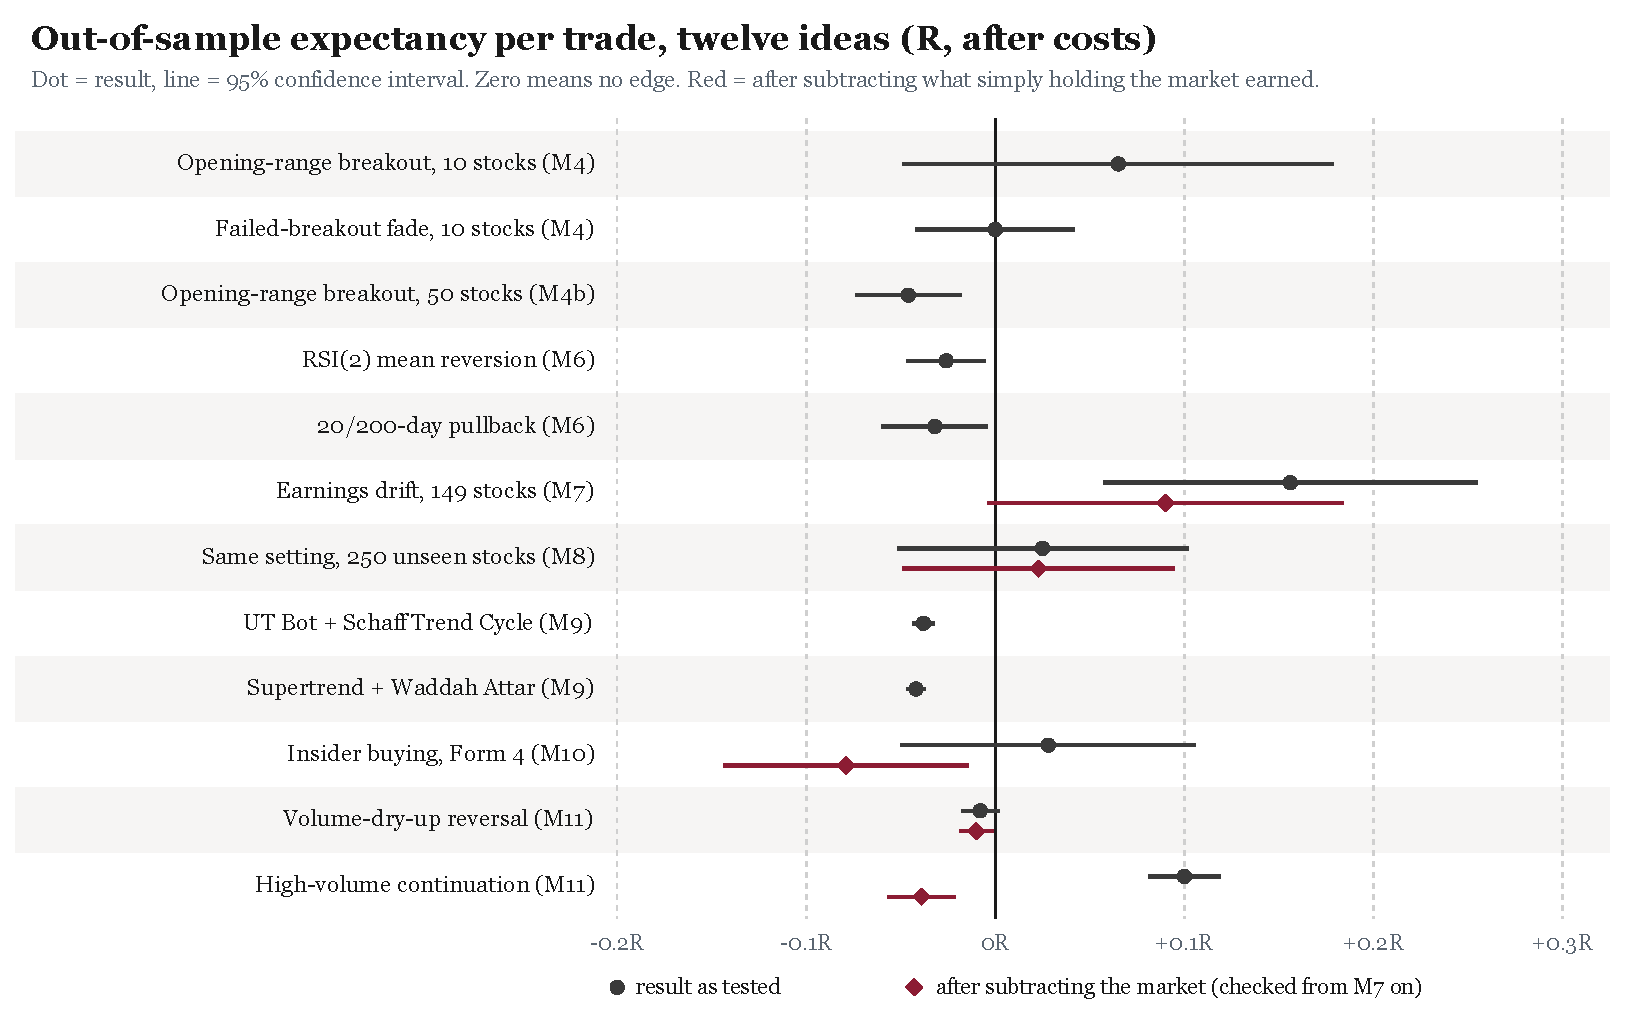
\includegraphics[width=1.0\linewidth]{figures/forest.pdf}
\caption[Out-of-sample result per trade, in R (profit measured in units of the amount risked)]{Out-of-sample result per trade, in R (profit measured in units of the amount risked). Zero means no edge. Blue: as tested. Orange: after subtracting what simply holding the market earned over the same dates, a check added from M7 on. Lines are 95\% confidence intervals.}
\label{fig:forest}
\figterms{M4 to M11 = the milestone numbers of the tests (see Table \ref{tbl:results}). RSI(2) = Relative Strength Index over 2 days, a gauge of very short-term momentum. 20/200-day = the 20-day and 200-day moving averages of the price. UT Bot = a trailing-stop trend indicator popular on charting sites; Schaff Trend Cycle (STC) = a momentum-cycle indicator. Supertrend = a trend line built from the average daily price range; Waddah Attar = a momentum-surge indicator. Form 4 = the SEC filing in which company insiders report their trades. Earnings drift = a stock keeps moving after its earnings reaction.}
\end{figure}

M12 is an event study (average market-adjusted return over five sessions, net of 10 basis points), not a strategy sweep,
so it has its own four criteria. ``M4'' and ``M4b'' are the ten-stock and fifty-stock runs of the same breakout grid.

Details, protocols and per-year numbers for each row are in \texttt{docs/m*-protocol.md} and \texttt{docs/m*-results.md}.

\subsection{Reading the table}\label{reading-the-table}

Each row is one test, run once. The result column is the average out-of-sample R per trade with its 95\% interval, and the last
column counts the pre-registered checks passed (six, or seven from M8 on). Three patterns stand out:

\begin{itemize}
\tightlist
\item
  \textbf{Intervals shrink with the number of trades.} The two indicator bots (M9) had about 100,000 trades each and intervals of
  ±0.005R, so their small negative results are firm. The ten-stock breakout (M4) had 435 trades and an interval of ±0.114R,
  wide enough to hide almost anything.
\item
  \textbf{Positive is not the same as significant.} Only two ideas had an interval entirely above zero before the market was
  subtracted: earnings drift (M7) and high-volume continuation (M11).
\item
  \textbf{Most failures were not close calls.} Seven of the twelve ideas passed only the minimum-trade-count check.
\end{itemize}

\subsection{Which safeguard stopped each idea}\label{which-safeguard-stopped-each-idea}

Table \ref{tbl:matrix} shows, for the twelve strategy tests, which pre-registered check each idea passed (yes) or failed (no); the columns
follow the seven checks of Section \ref{sec:method}. A dash means the check did not exist yet: the market-adjusted comparison was added after
earnings drift (M7).

\begin{table}[tbp]
\centering
\caption{Which pre-registered check each idea passed (yes) or failed (no); a dash means the check did not exist yet.}\label{tbl:matrix}
\begin{tabular}{@{}
  >{\raggedright\arraybackslash}p{(\linewidth - 14\tabcolsep) * \real{0.3226}}
  >{\raggedright\arraybackslash}p{(\linewidth - 14\tabcolsep) * \real{0.0968}}
  >{\raggedright\arraybackslash}p{(\linewidth - 14\tabcolsep) * \real{0.0968}}
  >{\raggedright\arraybackslash}p{(\linewidth - 14\tabcolsep) * \real{0.0968}}
  >{\raggedright\arraybackslash}p{(\linewidth - 14\tabcolsep) * \real{0.0968}}
  >{\raggedright\arraybackslash}p{(\linewidth - 14\tabcolsep) * \real{0.0968}}
  >{\raggedright\arraybackslash}p{(\linewidth - 14\tabcolsep) * \real{0.0968}}
  >{\raggedright\arraybackslash}p{(\linewidth - 14\tabcolsep) * \real{0.0968}}@{}}
\toprule
\begin{minipage}[b]{\linewidth}\raggedright
Idea
\end{minipage} & \begin{minipage}[b]{\linewidth}\raggedright
Enough trades
\end{minipage} & \begin{minipage}[b]{\linewidth}\raggedright
Above zero
\end{minipage} & \begin{minipage}[b]{\linewidth}\raggedright
Deflated Sharpe
\end{minipage} & \begin{minipage}[b]{\linewidth}\raggedright
Years
\end{minipage} & \begin{minipage}[b]{\linewidth}\raggedright
2x costs
\end{minipage} & \begin{minipage}[b]{\linewidth}\raggedright
Neighbours
\end{minipage} & \begin{minipage}[b]{\linewidth}\raggedright
Market-adjusted
\end{minipage} \\
\midrule
Opening-range breakout (M4) & yes & no & no & yes & yes & no & - \\
Failed-breakout fade (M4) & yes & no & no & no & no & no & - \\
Opening-range breakout, 50 stocks (M4b) & yes & no & no & no & no & no & - \\
RSI(2) mean reversion (M6) & yes & no & no & no & no & no & - \\
20/200-day pullback (M6) & yes & no & no & no & no & no & - \\
Earnings drift (M7) & yes & yes & no & yes & yes & yes & - \\
Earnings drift, replicated (M8) & yes & no & no & no & yes & no & no \\
UT Bot + Schaff Trend Cycle (M9) & yes & no & no & no & no & no & - \\
Supertrend + Waddah Attar (M9) & yes & no & no & no & no & no & - \\
Insider buying (M10) & yes & no & no & no & yes & yes & no \\
Volume-dry-up reversal (M11) & yes & no & no & no & no & no & no \\
High-volume continuation (M11) & yes & yes & no & yes & yes & yes & no \\
\bottomrule
\end{tabular}
\end{table}

Two checks did most of the work. Every idea had enough trades, but none passed the Deflated Sharpe check, and none of the
four ideas tested against the market passed that comparison. The interval check alone would have let two ideas through; the
market-adjusted comparison removed the rest of their gain. The M12 event studies and the M13 trend filter have their own
criteria and are not in the matrix.

\subsection{The two event studies (M12)}\label{the-two-event-studies-m12}

M12 asks a simpler question than the strategy tests: after the news, is any average move left to trade? For each event the
study enters at the first open at which the news could be traded (a post before 09:30 New York time at that day's open, any
other post at the next open, and a contract award at the open two sessions after its date, to err on the side of caution). It
holds five sessions, subtracts what SPY did over the same dates and 10 basis points of cost, and flips the sign for a negative
post. Four criteria were fixed in advance: at least 100 events; a positive average whose 97.5\% interval lies above zero; a
positive average in two thirds of the years with at least eight events; and a positive average in both halves of the sample.

Posts failed all but the first (average −0.05\%, positive in only 2 of 6 years); awards also failed all but the first (average
−0.10\%, positive in 5 of 9 years). Splitting the posts by tone changed little: positive posts averaged −0.01\% and negative
posts −0.12\%, where a negative number means the trade direction was wrong.

\section{Discussion: what kept recurring}\label{sec:discussion}

\begin{figure}[tbp]
\centering
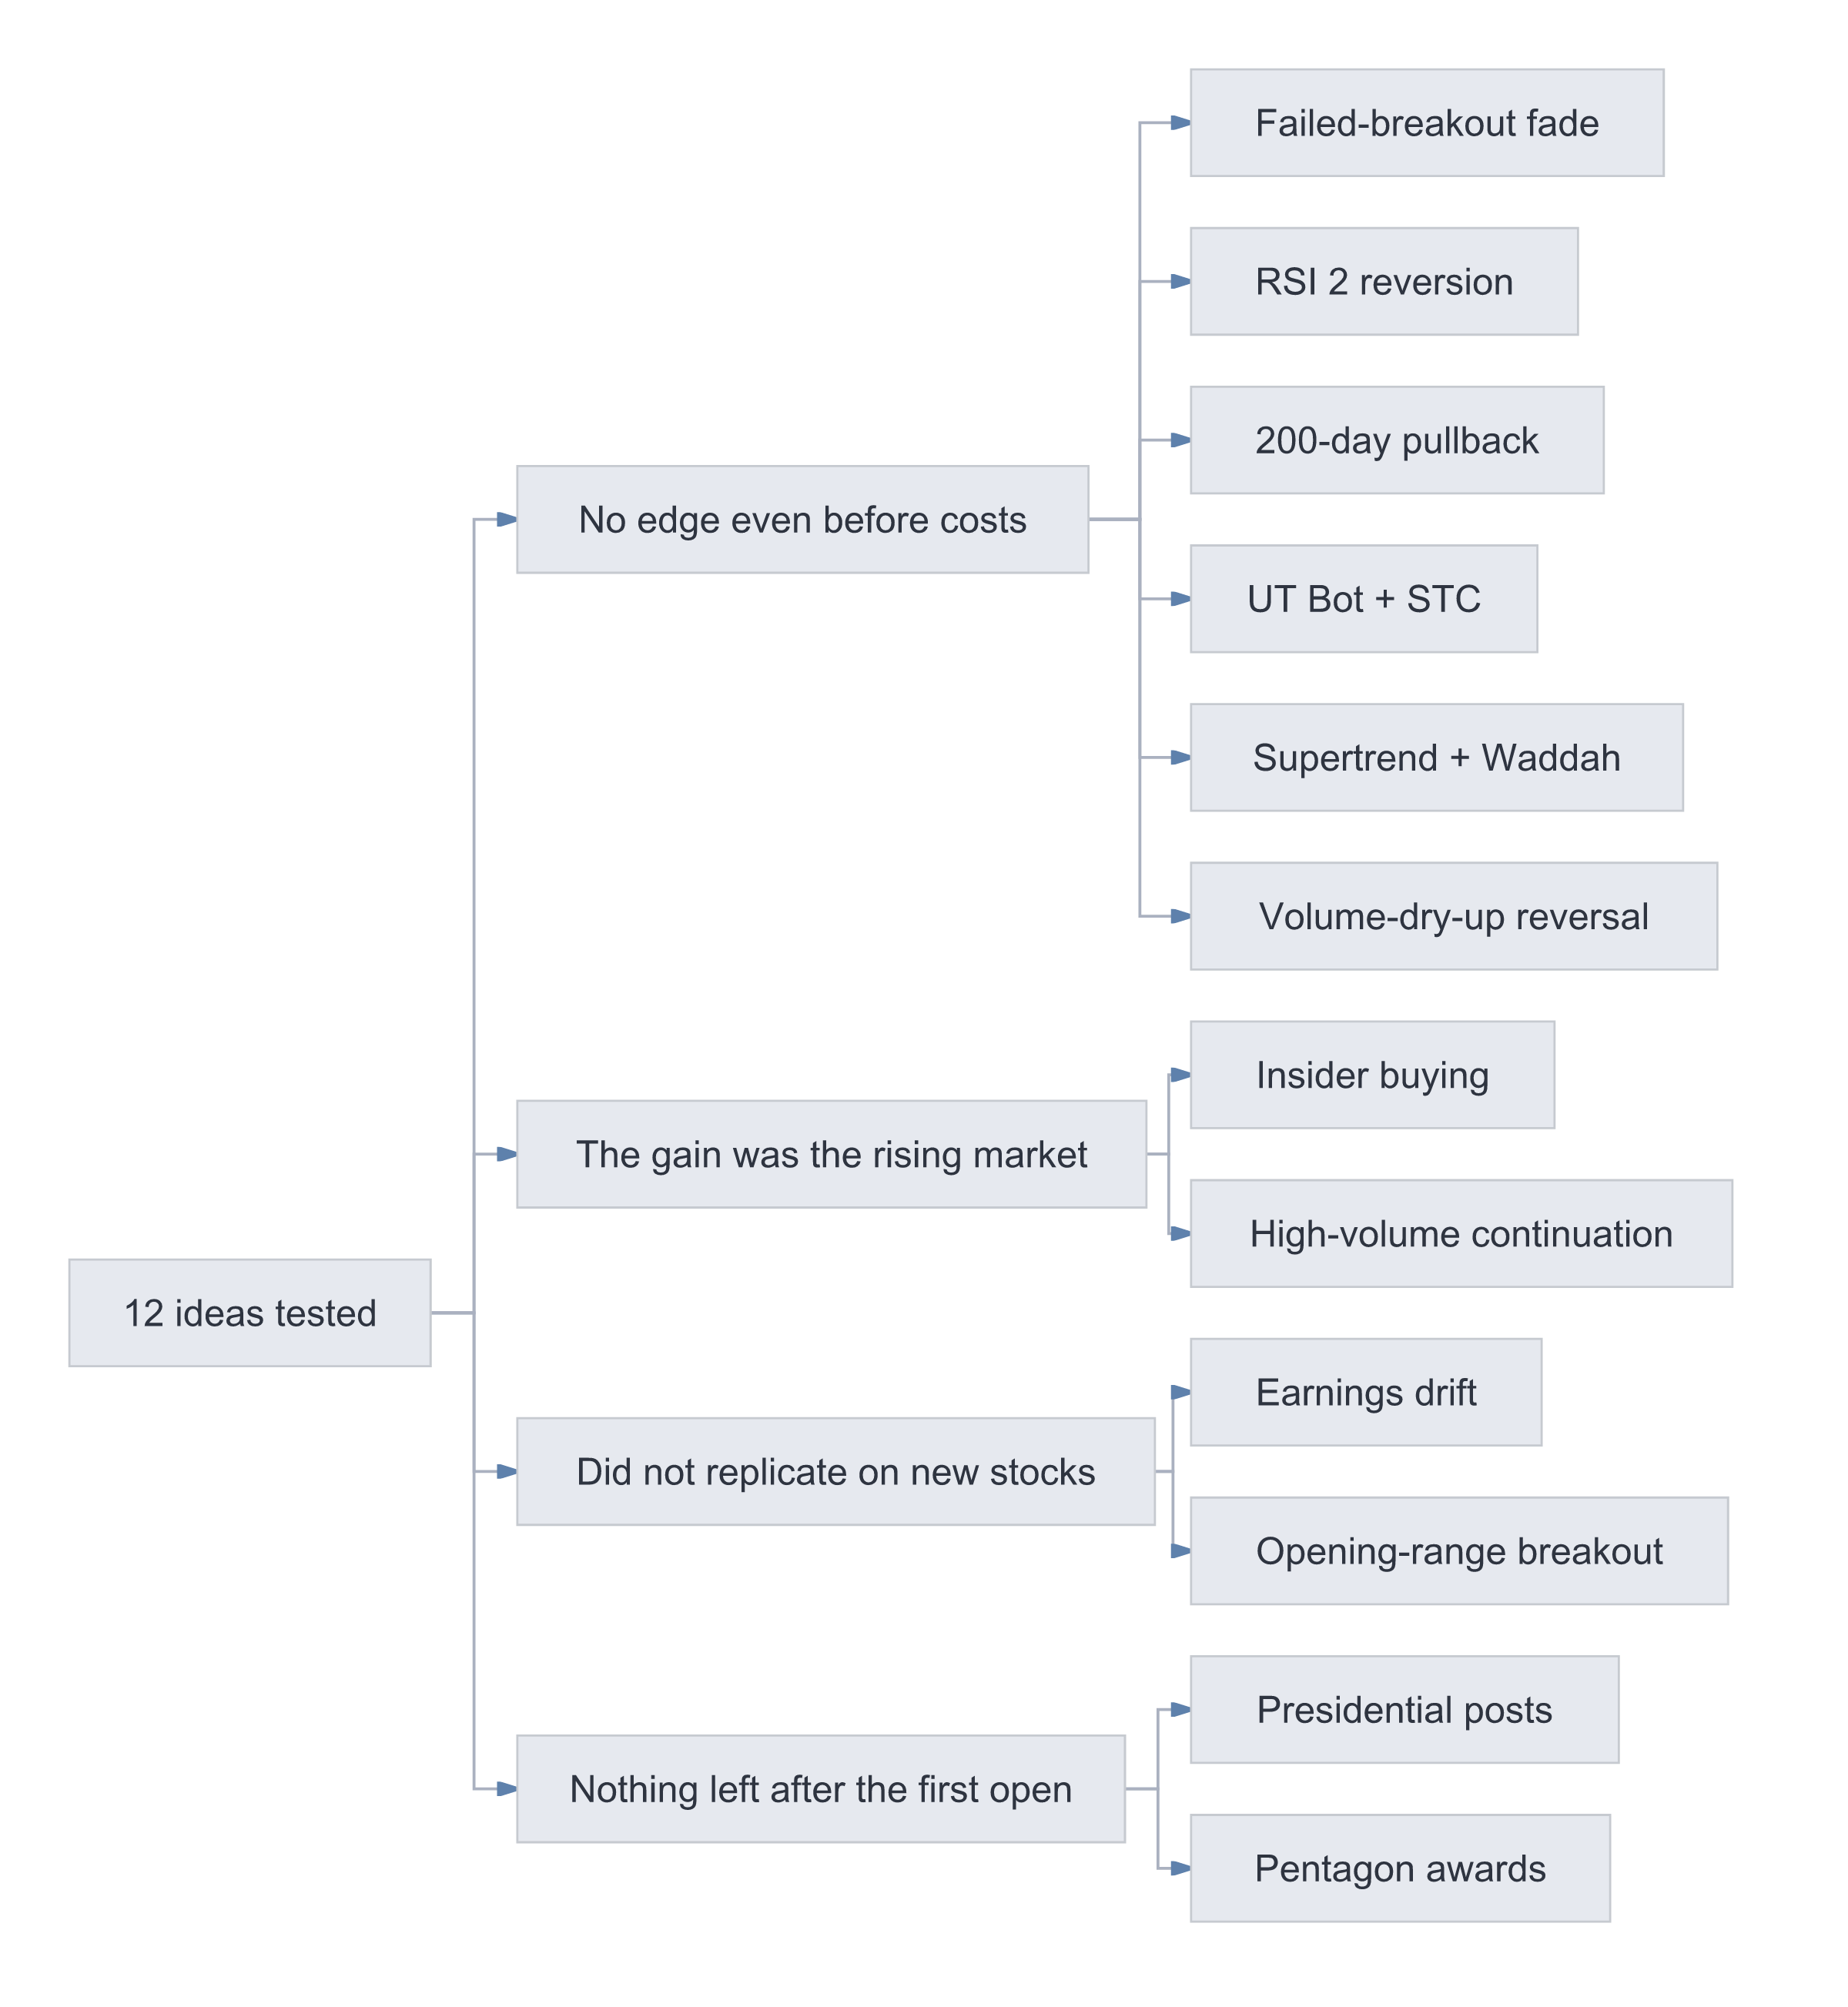
\includegraphics[width=0.98\linewidth]{figures/verdicts.png}
\caption[Why each idea failed, by main reason]{Why each idea failed, by main reason. Several had more than one: the breakout, for example, also showed a faint edge on 10 stocks that vanished on 50.}
\label{fig:verdicts}
\figterms{Before costs = the test was repeated with trading costs set to zero and still showed no gain. RSI 2 = 2-day Relative Strength Index. UT Bot = a trailing-stop trend indicator; STC = Schaff Trend Cycle, a momentum-cycle indicator. Supertrend = a trend line built from the average daily price range; Waddah = the Waddah Attar Explosion momentum indicator. Pullback = a dip back to a moving average inside a trend. Rising market = the gain disappeared once the market's own return was subtracted. New stocks = stocks that took no part in choosing the setting.}
\end{figure}

\textbf{Costs were not the explanation.} The first guess was that a one-cent spread against tight five-minute stops ate a
small edge. A zero-cost diagnostic showed otherwise: breakouts were −0.020R ±0.028 before costs and volume reversal
+0.006R ±0.010. There was no gross edge to eat, so cheaper execution would not have rescued these ideas.

\textbf{The market did the work.} The long-only families look strongest in 2019 to 2024, a period in which US stocks rose. The
market-adjusted check changed the picture (Table \ref{tbl:market}):

\begin{table}[tbp]
\centering
\caption{The three strongest long-side results, before and after subtracting the market.}\label{tbl:market}
\begin{tabular}{@{}lll@{}}
\toprule
Idea & As tested & After subtracting the market \\
\midrule
Earnings drift (M7) & +0.156R & +0.090R ±0.094 \\
Insider buying (M10) & +0.028R & −0.079R ±0.065 \\
High-volume continuation (M11) & +0.100R & −0.039R ±0.018 \\
\bottomrule
\end{tabular}
\end{table}

All 16 volume-spike configurations were positive as tested, and they still failed. A related effect: the stock universe is
made of companies that were liquid in 2016 and are still listed today. Survivors make long positions look better and short
positions worse (in M6 longs were near zero and shorts clearly negative).

\textbf{Lucky results did not replicate.} The ten-stock breakout test (+0.065R) turned into −0.046R on fifty fresh stocks, with
all 54 configurations negative. Earnings drift passed five of six checks and then fell to +0.025R on 250 unseen stocks.
The Deflated Sharpe check had flagged the first of these in advance; replication confirmed it.

\textbf{Several attractive stories went nowhere.} Distinguishing routine from opportunistic insider trades follows a well-known
paper \cite{cohen2012};
in our large and mid-cap universe there were too few opportunistic buys to test the split. Presidential posts: published
work finds same-day reactions to tweets about firms
\cite{ajjoub2021}, but starting at the next
open, as a slower trader must, nothing was left.

\subsection{A closer look: the near miss}\label{a-closer-look-the-near-miss}

Earnings drift came closest, so it is worth following step by step. On 149 liquid stocks it passed five of six checks: 551
trades, +0.156R ±0.099, positive in all six years and still positive at double costs. Only the Deflated Sharpe check failed
(0.006), because the winning setting was one of 36 tried. About half of the raw gain was the rising market (+0.090R after
subtracting it), and the drift appeared only from 2019 on. The test that settles such a case is replication: the same setting,
frozen, on 250 stocks that had played no part in choosing it. There the average fell to +0.025R ±0.077 (+0.023R after the
market), the year-by-year results turned into noise (+0.06, −0.06, −0.07, +0.12, +0.20 and −0.07R), and the measured drift
in the price reaction itself shrank from +1.13\% to +0.06\%.

\section{A side question: does a trend filter make holding the market safer?}\label{sec:trend}

Since the market kept beating the rules, I tested the simplest allocation rule: hold SPY while it is above its 200-day
average, otherwise hold cash. One parameter, fixed in advance, 2017 to 2024 (Table \ref{tbl:trend}):

\begin{table}[tbp]
\centering
\caption{Holding SPY with and without the 200-day trend filter, 2017 to 2024.}\label{tbl:trend}
\begin{tabular}{@{}lll@{}}
\toprule
& Buy and hold & 200-day filter \\
\midrule
Return per year & 12.8\% & 8.8\% \\
Worst drawdown & −32.4\% & −21.8\% \\
Sharpe (risk-adjusted, no cash yield) & 0.78 & 0.75 \\
\bottomrule
\end{tabular}
\end{table}

It reduced the worst falls (2020: −19\% instead of −32\%; 2022: −17\% instead of −27\%) but missed the rebounds, and 18
of its 26 in-and-out trades lost money. It passed two of three pre-registered checks and failed the return one by
about 4 points a year. Eight years and two crashes are a short sample, and this is research, not advice: how large a fall
a holder can sit through matters more than these figures.

\section{Limitations}\label{sec:limits}

Absence of evidence in these tests is not proof that no edge exists. The scope was narrow:

\begin{itemize}
\tightlist
\item
  \textbf{Free data and daily or five-minute bars.} I could not test the first seconds and minutes after news, where fast
  traders operate, nor order-book or options data, nor paid datasets (earnings estimates, short interest, intraday news).
\item
  \textbf{Large and mid caps only.} Several published effects are strongest in small stocks. I could not test them honestly
  because free price history omits delisted companies, which biases any such result upward.
\item
  \textbf{One regime.} 2016 to 2024 is one stretch of one market, dominated by a rise. The holdout (2025 onward) was kept unread
  for a final run that no idea earned.
\item
  \textbf{Survivor and hindsight bias.} The universe is stocks listed today. This was disclosed in each protocol and is why the
  market-adjusted check matters.
\item
  \textbf{Clustering.} Events bunch in market selloffs, so confidence intervals are somewhat optimistic about independence.
\item
  \textbf{Backtests are not live trading.} Slippage in fast markets, rejected orders and partial fills are modelled
  approximately. A paper-trading loop was built and tested against a broker's paper account for plumbing only; nothing was
  run for evidence.
\end{itemize}

\section{Conclusion}\label{sec:conclusion}

\begin{itemize}
\tightlist
\item
  \textbf{No idea passed.} Of twelve, the closest were earnings drift (5 of 6 checks, then it failed to replicate on 250
  unseen stocks) and a volume-spike rule (5 of 7 checks, then it turned negative after subtracting the market).
\item
  \textbf{When it looked like an edge, it was mostly the market.} Long-only rules were positive in 2019 to 2024 largely
  because stocks rose. Insider buying went from +0.028R to −0.079R, and volume spikes from +0.100R to −0.039R, once the
  market was subtracted.
\item
  \textbf{Costs were not the main reason.} The price-pattern families had no edge even at zero cost (for example breakouts at
  −0.020R, volume reversal at +0.006R, both consistent with zero).
\item
  \textbf{Replication was the strongest filter.} A faint breakout result on 10 stocks (+0.065R) became −0.046R on 50 fresh
  ones. Earnings drift (+0.156R) became +0.025R on 250 unseen stocks.
\item
  \textbf{Precision was high, so the negatives are real.} Some tests had around 100,000 trades with intervals of about
  ±0.005R. These are measured zeros and small negatives, not ``not enough data''.
\item
  \textbf{A side question gave a trade-off, not a free lunch.} A 200-day trend filter on SPY cut the worst drawdown from −32\% to
  −22\% but cost about 4 points a year of return.
\end{itemize}

\section{Recommendations}\label{sec:recommendations}

\begin{enumerate}
\def\labelenumi{\arabic{enumi}.}
\tightlist
\item
  \textbf{Write the rules down before you look.} Commit them. It removes the most common way to fool yourself.
\item
  \textbf{Count your tries.} The best of many looks good by luck; deflate for it.
\item
  \textbf{Subtract the market.} In a rising period a long-only rule needs to beat holding, not zero.
\item
  \textbf{Replicate on stocks that took no part in choosing the rule.} It was the strongest filter here.
\item
  \textbf{Ask whether there is a gross edge before blaming costs.}
\item
  \textbf{Treat screenshots, reels and ``I made X overnight'' posts as hypotheses.} They are one run, picked after the fact, and
  rarely come with losing runs or costs. They deserve the same test as anything else, and most will fail it.
\item
  \textbf{A clear ``no'' is a result.} It saved capital, and the method now makes the next question cheap to test.
\end{enumerate}

\section{Reproducibility}\label{sec:repro}

Everything is in the project repository: code, each protocol (committed before its run), each result write-up and the tests
(208 passing). Data is not redistributed; the scripts fetch it from the free sources above.

\begin{verbatim}
uv sync
uv run pytest
uv run python scripts/sweep.py --config config/sweeps/m10-insider.toml
\end{verbatim}

The last command reruns one pre-registered sweep (insider buying).

Start with \texttt{README.md}, then \texttt{docs/m4-protocol.md} for the method and \texttt{docs/m*-results.md} for each result.

% ================================================================ appendices
\appendix
\renewcommand{\thesection}{\Alph{section}}

\section{Glossary}\label{app:glossary}

Every abbreviation and technical term used in the paper, in alphabetical order.

\begin{description}[style=sameline,leftmargin=4.4cm,labelwidth=4.2cm,labelsep=0.2cm,font=\sffamily\bfseries\small\color{accent},itemsep=3pt]
  \item[ADX] Average Directional Index: a measure of how strongly a market is trending.
  \item[ATR] Average True Range: the typical daily price range of a stock, used to size stops.
  \item[Backtest] Replaying historical data to see what a fixed rule would have done.
  \item[Bar] A price candle for one period: open, high, low, close and volume.
  \item[Basis point (bp)] One hundredth of one percent (0.01\%).
  \item[Choppiness Index] A measure of whether a market is ranging rather than trending.
  \item[Confidence interval] The range in which the true average very probably lies; here 95\% unless stated.
  \item[Deflated Sharpe Ratio] The probability that the best Sharpe ratio is genuine after accounting for the number of tries.
  \item[EDGAR] The SEC's public database of company filings.
  \item[Event study] Measuring the average price move after a type of event, such as an earnings release.
  \item[Expectancy] The average result per trade, here in R.
  \item[Form 4 / 8-K] SEC filings: insider trades (Form 4) and material company events such as earnings (8-K, Item 2.02).
  \item[Holdout] Recent data (2025 onward) kept unread for a single final test.
  \item[Out of sample] Data that played no part in choosing a rule's settings.
  \item[Paper trading] Simulated trading on a broker's practice account, with no real money.
  \item[Pre-registration] Writing down and committing the rules and pass criteria before running a test.
  \item[R] Profit measured as a multiple of the amount risked on the trade.
  \item[RSI] Relative Strength Index: a gauge of recent momentum; RSI(2) uses two days.
  \item[SEC] The US Securities and Exchange Commission.
  \item[Sharpe ratio] Average return divided by its volatility: return per unit of risk.
  \item[Slippage] The cost of trading at a worse price than the last quote, assumed per share.
  \item[SPY] An exchange-traded fund that tracks the S\&P 500 index; used as ``the market''.
  \item[STC] Schaff Trend Cycle: a momentum-cycle indicator.
  \item[Supertrend] A trend line built from the average true range.
  \item[Survivorship bias] Distortion from studying only companies that still exist today.
  \item[UT Bot] A trailing-stop trend indicator popular on charting sites.
  \item[Waddah Attar Explosion] A momentum-surge indicator with a dead zone based on ATR.
  \item[Walk-forward] Choosing settings on earlier years and judging them on the next, year by year.
\end{description}

\section{Index of protocols and results}\label{app:index}

Each test has a protocol, committed before the run, and a result write-up, in the \texttt{docs} folder of the repository.

\begin{table}[H]
\centering
\caption{Where to find each test's protocol and result.}\label{tbl:index}
\begin{tabular}{@{}>{\raggedright\arraybackslash}p{0.09\linewidth}>{\raggedright\arraybackslash}p{0.39\linewidth}>{\raggedright\arraybackslash}p{0.25\linewidth}>{\raggedright\arraybackslash}p{0.21\linewidth}@{}}
\toprule
Test & Idea & Protocol & Result \\
\midrule
M4 & Opening-range breakout, failed-breakout fade & m4-protocol.md & m4-results.md \\
M4b & Breakout on 50 fresh stocks & m4b-protocol.md & m4b-results.md \\
M6 & RSI(2) reversion, 20/200-day pullback & m6-swing-protocol.md & m6-results.md \\
M7 & Earnings-announcement drift & m7-events-protocol.md & m7-results.md \\
M8 & The same setting on 250 unseen stocks & m8-confirmation-protocol.md & m8-results.md \\
M9 & UT Bot + STC, Supertrend + Waddah Attar & m9-indicators-protocol.md & m9-results.md \\
M10 & Insider buying & m10-insider-protocol.md & m10-results.md \\
M11 & Volume reversal and continuation & m11-volume-protocol.md & m11-volume-results.md \\
M12 & Presidential posts, Pentagon awards & m12-political-protocol.md & m12-political-results.md \\
M13 & 200-day trend filter on SPY & m13-trend-filter-protocol.md & m13-trend-filter-results.md \\
\bottomrule
\end{tabular}
\end{table}

M0 to M3 and M5 are infrastructure: decisions, a data-depth probe, the recorder, the backtest engine and the
paper-trading loop.

\section*{Disclosures}
\addcontentsline{toc}{section}{Disclosures}
\markboth{Disclosures}{}

This is a personal research project. It is not investment advice and recommends no security or strategy. No real money was
traded. The code, analysis and drafting were done with an AI coding assistant (Claude Code); every number in this paper is
taken from results recorded in the repository, and the protocols' commit order is the evidence of what was decided when.

% ================================================================ references
\renewcommand{\refname}{References}
\begin{thebibliography}{9}
\addcontentsline{toc}{section}{References}
\bibitem{bailey2014} D.~H. Bailey and M. L\'opez de Prado, ``The Deflated Sharpe Ratio: Correcting for Selection Bias,
  Backtest Overfitting, and Non-Normality,'' \emph{Journal of Portfolio Management}, 40(5), 2014.
  \url{https://papers.ssrn.com/abstract=2460551}
\bibitem{cohen2012} L.~Cohen, C.~Malloy and L.~Pomorski, ``Decoding Inside Information,'' \emph{Journal of Finance},
  67(3), 1009--1043, 2012. \url{https://econpapers.repec.org/RePEc:bla:jfinan:v:67:y:2012:i:3:p:1009-1043}
\bibitem{ajjoub2021} C.~Ajjoub, T.~Walker and Y.~Zhao, ``Social media posts and stock returns: The Trump factor,''
  \emph{International Journal of Managerial Finance}, 17(2), 185--213, 2021.
  \url{https://econpapers.repec.org/RePEc:eme:ijmfpp:ijmf-02-2020-0068}
\bibitem{martineau2022} C.~Martineau, ``Rest in Peace Post-Earnings Announcement Drift,'' \emph{Critical Finance Review},
  11(3--4), 613--646, 2022. \url{https://econpapers.repec.org/RePEc:now:jnlcfr:104.00000122}
\end{thebibliography}

\end{document}
